\chapter{Numbers}
\label{ch:numbers}

\chapquote{He who refuses to do arithmetic is doomed to talk nonsense.}{John McCarthy, American computer scientist}

%\chapquote{God made the integers, all the rest is the work of man.}{Leopold Kronecker, German mathematician}

The number system that we use every day, both in mathematics class and in our regular lives, developed over many generations. Men and women from all over the world, both famous and anonymous, have helped to make mathematics what it is today.

People argue over whether mathematical ideas are ``invented'' or ``discovered''. For example: \glspl{imaginary number} (which we will discuss briefly in Algebra 1, and study in more detail in Algebra 2), first appeared on the mathematical scene in the 1500s. Italian mathematician Gerolamo Cardano wrote about these new numbers in his work with certain types of problems that otherwise would have been impossible to solve. Since he was one of the first people to describe this new kind of number, we might say that Cardano \textit{invented} imaginary numbers.

But, we now know that imaginary numbers have practical applications in, for example, electrical engineering. The laws of electromagnetism haven't changed since the 1500s. (Well, our understanding of the laws has changed, but the physics has not.) So, maybe imaginary numbers have been there all along, lurking within the fabric of the universe. In this case, Cardano \textit{discovered} imaginary numbers.

It's not clear which is the more accurate description. No matter what side of the debate you find more convincing, there is a certain beautiful interconnectedness to our system of numbers and mathematical laws. To illustrate this, we'd like to tell a story.

% % % % % % % % % % % % % % % % % % % % % % % % % % % % % % % % % % % % % % % % 
\section{Story of numbers}
\label{sec:storyofnumbers}

%%%
\newenvironment{story}
{\begin{slshape}}
{\end{slshape}}
%%%

\begin{story}
Once upon a time, there was a simple farmer. Knut Krumbli lived in rural Sweden, raising goats and making goat cheese. He and his family led an uncomplicated life, and they didn't have much need for mathematics. In fact, they really only needed numbers to count their goats: 1 goat, 2 goats, 3 goats, 4 goats\ldots

But one day, after a terrible storm, Knut went to the field to count the goats and discovered, much to his dismay, that there were no goats to count. He hadn't needed a number to describe this situation before, but now people were asking him hard questions, like ``How many of your goats made it through that crazy storm?'' (But, you know, in Swedish.)

Knut and his family couldn't very well survive without any goats, so he went to his neighbor for help. The neighbor agreed to loan Knut some goats to restart his herd, but, of course, Knut would have to repay his goat-debt later. The village hadn't needed to do much accounting before the storm, but now they needed a system of numbers that could keep track of debts and credits.

Over time, Knut's family got back on their feet and thrived. They paid back their debts and eventually grew to raise more goats and to make more goat cheese than they could eat. They began to trade with their neighbors for other goods or services. Of course, everything had relative value: three wheels of goat cheese were worth two bales of hay. So, the village developed a system of numbers for describing exchange rates of this kind.

As the village grew, Knut's family farm led the development of a booming goat cheese industry. They invested their profits into bank accounts that paid interest. In certain situations, everyone was surprised to discover, interest-bearing accounts led to a new system of numbers that no one had seen before.

Eventually, some of Knut's ancestors emigrated to America and, years later, a pair of twins -- Knut's great-great-great-grandchildren -- would grow up to change the world. But let's not get too far ahead of ourselves. More about the Krumbli twins later\ldots
\end{story}

\kverse{Meet Knut Krumbli, great-great-great-grandfather, Swedish goat farmer.}

\subsection{Dissecting the story}

It's natural to begin our discussion of numbers exactly where Knut began: counting things. The numbers we use to count are called the \glspl{natural number} (also known as the counting numbers, for obvious reasons).

\begin{boxdef}[Natural number]
A member of the list of numbers that starts $1, 2, 3, 4,\dotsc$ and continues forever. The set of all natural numbers is denoted using the symbol $\N$, so we can write \[\N = \{1, 2, 3, 4, \dotsc\}.\]
We use the \{curly braces\} here to indicate that we're collecting a group of numbers together as a \gls{set}. A set written in this way is written in \gls{set notation}.
\end{boxdef}

The natural numbers have some interesting properties. If we add two natural numbers, their sum will always be a natural number. The same goes for multiplication: the product of two natural numbers is again a natural number.

Mathematically speaking, we call this \gls{closure}. We say that the natural numbers are closed under the operation of addition. Also, the natural numbers are closed under the operation of multiplication.

Notice that we didn't include 0 among the natural numbers. Zero is a bit tricky because it seems like a counting number. For example, ``zero'' is (probably) the answer to the counting question, ``How many goats are there in the room with you right now?'' But if there are no goats to count, can we really count them? That's a philosophical question.\footnote{Philosophy and mathematics have historically gone hand-in-hand. Many important discoveries (inventions?) in mathematics are attributed to people who are considered both ``philosopher'' and ``mathematician''. For example: French mathematician Ren\'{e} Descartes, for whom the Cartesian coordinate system is named, is also the philosopher who said ``I think therefore I am''.}

Practically speaking, we usually exclude 0 from the set of natural numbers. We will always be very clear when we come to situation where we want to consider 0 to be a natural number.

The natural numbers are closed under the operations of addition and multiplication, but they are \textit{not} closed under the operation of subtraction. Sometimes, the difference of two natural numbers is a natural number: for example $8-6=2$, no problem. But some subtraction sentences don't work: for example $10-13 = \umin3$, and $\umin3$ is not a natural number. In cases like this, we don't have a natural number, but an \gls{integer}.

\begin{boxdef}[Integer]
A natural number, or the opposite of a natural number, or zero. The set of all integers is denoted $\Z$, so we sometimes write \[\Z = \{\dotsc, \umin3, \umin2, \umin1, 0, 1, 2, 3, \dotsc \}.\]
We could also write $\Z = \{0, \pm1, \pm2, \pm3, \dotsc\}$.

The symbol $\Z$ comes from \textit{Zahl}, the German word for number.
\end{boxdef}

Note that every natural number is an integer. We say that the set of natural numbers is a \gls{subset} of the set of integers.\footnote{For those who are into mathematical symbols and notation, the sentence ``The natural numbers are a subset of the integers'' is denoted $\N \subseteq \Z$.}

The integers are closed under the operations of addition and multiplication. Plus -- bonus! -- the integers are closed under the operation of subtraction. Whenever we subtract one integer from another, we always get another integer as the result.

But (as you may have noticed) we have a problem with division. In certain cases, the quotient of two integers is itself an integer: $15 \div \umin3 = \umin5$, no problem. But other times we get a quotient that is not an integer: $\umin3 \div 15 = \umin0.2$ and $\umin0.2$ is not an integer. In other words, the integers are not closed under the operation of division. To achieve closure under division, we must turn to the \gls{rational number}.

\begin{boxdef}[Rational number]
\label{def:rationals}
Any number that can be written as the ratio of two integers $\frac{a}{b}$, where $b$ is not zero. This set includes all of your classic fractions, as well as all terminating decimals and all repeating decimals.

%The set of all rational numbers is denoted $\Q$, so we sometimes write \[\Q = \left\{ \tfrac{a}{b} \text{ where $a$ and $b$ are integers, and $b \neq 0$} \right\}\] 

The set of all rational numbers is denoted by the symbol $\Q$, which comes from the word \textit{quotient}.
\end{boxdef}

%\footnote{Fractions, the F-word of mathematics?}
Fractions have a lousy reputation among math students, but the rational numbers are great because they are closed under all four of the basic operations. When we add, subtract, multiply, or divide any two rational numbers, the result will always be another rational number. What more could we ask for? In some sense, $\Q$ is a complete number system, and in fact the world was content with the rational numbers for a long time.

But, other numbers exist. Yes, the rational numbers include all of the terminating decimals (like $0.5$ and $1.678$), and all of the repeating decimals (like $0.\overline{3}$ and $\umin12.34\overline{56}$). But consider the number \[0.10\,110\,1110\,11110\,111110\ldots\] This number does not terminate, but it does not repeat either.\footnote{This number does have a pattern, but that is not the same as ``repeating'' in the sense of ``repeating decimal''. In a repeating decimal the same digit or group of digits recurs over and over again.} So, this number is \textit{not} a rational number. It is an \gls{irrational number}.

\begin{boxdef}[Irrational number]
A number that cannot be expressed as the ratio of two integers. In decimal form, an irrational number never terminates and never repeats.
\end{boxdef}

You have likely encountered irrational numbers before. A famous example is the number $\pi$ (pi), which shows up when we study circles. We usually approximate $\pi$ to be about $3.14$, but in fact the decimal representation of $\pi$ goes on forever without stopping or repeating.\footnote{We use the symbol $\approx$ to mean ``is approximately equal to''. We write $\pi\approx3.14$ and not $\pi=3.14$, because 3.14 is only an approximation of $\pi$, not its exact value.}
\[\pi \approx 3. 141\,592\,653\,589\,793\,238\,462\,643\,383\,279\,502\,884\,197\,693\,993\,751\,058\,209\,749\,445\,923\,078\,164\ldots\]

When we group together all of the rational numbers and all of the irrational numbers, we will have accounted for all possible decimal representations. This combined set of numbers, called the \glspl{real number}, is going to be of key importance to us in Algebra 1.

\begin{boxdef}[Real number]
Any rational or irrational number. The set of all real numbers is denoted $\R$ which, naturally enough, comes from the word \textit{real}.
\end{boxdef}

Like the set $\Q$, the set $\R$ is closed under the four fundamental operations. $\Q$ and $\R$ are the number systems we will work with in Algebra 1. Other types and sets of numbers exist, like $\C$, the set of so-called \glspl{complex number}. Complex numbers will be a topic of study in Algebra 2, but we will spend our time in Algebra 1 with $\Q$ and $\R$.


% % % % % % % % % % % % % % % % % % % % % % % % % % % % % % % % % % % % % % % % 
\section{Integers}
\label{sec:integers}

You have probably been working with positive and negative numbers for a while now, so this section will review the most important terms and algorithms for signed numbers. To get the ball rolling, think about this:

\begin{boxexplore}[Integer comparisons]
In each of the expressions below, assume that $x$ and $y$ are natural numbers and that $x<y$ ($x$ is less than $y$). Will the result be greater than 0, less than 0, equal to 0, or is there not enough information to tell? Why?

\begin{tabularx}{\textwidth}{YYYY}
(a)\quad $x+(\umin y)$
&
(b)\quad $x-(\umin y)$
&
(c)\quad $x \cdot (\umin y)$
&
(d)\quad $x \div (\umin y)$
\end{tabularx}
\end{boxexplore}

\subsection{Language of signed numbers}

As we saw in \cref{sec:storyofnumbers}, the integers include the natural numbers, their opposites, and zero. Numbers now include two pieces of information: they have a \textit{size} (or \textit{magnitude}) and a \textit{direction}, either positive or negative.\footnote{Later in mathematics and the physical sciences, we'll encounter mathematical objects with both magnitude and direction again. They're called vectors.} Sometimes, we care only about the magnitude of a number, in which case we refer to a number's \gls{absolute value}.

\begin{boxdef}[Absolute value]
The absolute value of a number $x$ is its distance away from zero on the number line. To express this in mathematical symbols, we write $\abs{x}$ to mean ``the absolute value of $x$''.
\end{boxdef}

For those who like memory aids, it may be helpful to think of the absolute value bars as a little numerical shower stall or car wash: a number goes in and all its negativity gets washed away.

\begin{boxex}
\begin{enumerate}[itemsep=10pt]
\item \onerowex{$\abs{4}$}{The absolute value of a positive number is just the original number, so $\abs{4}=4$.}

\item \onerowex{$\abs{\umin8}$}{Absolute value ignores the sign and tells us how far a number is from zero. $\umin8$ is eight units away from zero, so $\abs{\umin8} = 8.$}

\item \onerowex{$\umin\abs{\umin6}$}{The absolute value bars only apply to what's inside, but then this negative sign \textit{outside} the absolute value bars will make the final answer negative again! So, $\umin\abs{\umin6} = \umin6$. Note that $\umin\abs{6}$ would also be $\umin6$.}
\end{enumerate}
\end{boxex}

Every nonzero number has a counterpart that is the same distance away from zero, but on the opposite side of the number line. This is a simple idea, but one that is important enough for us to give it a name.

\begin{boxdef}[Opposite]
The \gls{opposite} of a number $x$ is the number $-x$. In other words, the opposite of a number is the number with the \textit{same absolute value}, but the \textit{opposite sign}. For example, 3 and $\umin3$ are opposites. The number 0 is its own opposite.

\begin{center}
\begin{tikzpicture}
	\draw[fill=defcolor] (-3,0) circle[radius=0.1];
	\draw[fill=defcolor] (3,0) circle[radius=0.1];
	\draw[<->,thick] (-5.5,0) -- (5.5,0);
	\foreach \x in {-5,...,5} \draw (\x,0.1) -- (\x,-0.1) node[below]{\x};
\end{tikzpicture}
\end{center}
\end{boxdef}

The sum of opposites is always 0. For this reason, we sometimes use the term \gls{additive inverse} to describe the opposite of a number. (More on inverses in \cref{ch:equations}.)

\subsection{Adding signed numbers}
\index{addition!of signed numbers}

Like matter and antimatter, combining positive and negative numbers leads to annihilation.\footnote{Dramatic, no?} For example when we bring together $+8$ and $\umin6$, we can picture 8 units of ``matter'' and 6 units of ``antimatter''. Particles and antiparticles annihilate one another, both disappearing in the process. Since we have more matter than antimatter in this case, all of the antimatter is consumed, leaving behind 2 units of matter.

%\begin{center}
\begin{figure}[!htbp]
\centering
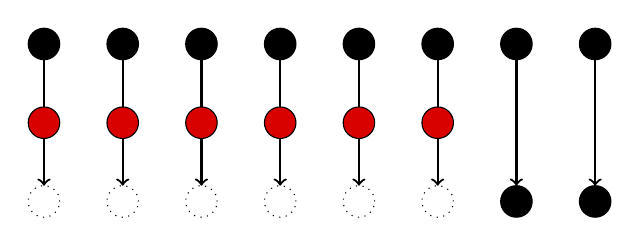
\begin{tikzpicture}
\foreach \x in {1,2,...,8} {
	\draw[fill] (\x,1) circle (0.2cm);
	\draw[->,thick] (\x,1) -- (\x,-0.8);
}
\foreach \x in {1,2,...,6} \draw[dotted] (\x,-1) circle (0.2cm);
\foreach \x in {1,2,...,6} \draw[fill=red!85!black] (\x,0) circle (0.2cm);
\draw[fill] (7,-1) circle (0.2cm);
\draw[fill] (8,-1) circle (0.2cm);
\end{tikzpicture}
\caption{Eight units of matter versus six units of antimatter.}
\label{fig:intadd}
\end{figure}
%\end{center}

We might visualize annihilation with a drawing like in \cref{fig:intadd} where black circles are units of matter, red circles are units of antimatter. Or, we could write a number sentence like $8 + \umin6 = 2$. Of course, no annihilations occur when we scrape together a big pile of matter (or a big pile of antimatter, for that matter). It's only when they mix that anything interesting happens.

\begin{boxdef}[Adding signed numbers]
When adding two numbers that have the same sign, we add the absolute values of the numbers, and use the sign that they share.

Otherwise, when adding two numbers that have different signs, we find the difference between their absolute values, and use the sign of the number with larger absolute value.
\end{boxdef}

\begin{boxex}
Compute each of the following.

\begin{enumerate}[itemsep=10pt]
%\item \onerowex{$8+12$}{We add as usual, like we've been doing since elementary school: $8+12=20$}

\item \onerowex{$\umin8 + \umin12$}{Both numbers are negative. That's a big pile o' antimatter: $\umin8+\umin12 = \umin20$}

\item \onerowex{$\umin8 + 12$}{The numbers have different signs, so prepare for annihilation! $\abs{12}$ is larger than $\abs{\umin8}$, so we will have matter left over. Therefore, $\umin8 + 12 = 4$}

%\item \onerowex{$8 + \umin12$}{This time, we have more antimatter than matter: $8+\umin12 =\umin4$}
\end{enumerate}
\end{boxex}

\subsection{Subtracting signed numbers}
\index{subtraction!of signed numbers}

Addition and subtraction are called \textit{opposite} (or \textit{inverse}) \textit{operations} because they ``undo'' one another. The act of adding 5 of matter can be ``undone'' by subtracting 5 units of matter. On the other hand, the act of adding 5 units of matter can also be undone by \textit{adding 5 units of antimatter}.

\begin{boxdef}[Subtracting signed numbers]
\textit{Subtracting a number} is the same as \textit{adding the opposite of the number}.

When faced with a subtraction problem, change it to an ``addition of the opposite'' problem and then follow the rules for adding signed numbers.
\end{boxdef}

The benefit of this approach is that we can avoid having to learn a whole new set of rules for subtracting signed numbers. All we need are the rules for addition, plus one new rule about how to change subtraction problems into addition problems!

\begin{boxex}
Compute each of the following:

\begin{enumerate}[itemsep=10pt]
\item \onerowex{$8-12$}{``Subtracting 12'' is the same as ``adding negative 12'', so $8-12=8+\umin12$. Then, we can apply the rules for adding signed numbers: $8+\umin12~=~\umin4$}

\item \onerowex{$\umin3 - 14$}{This is the same as $\umin3 + \umin14$, and we follow the rules for adding numbers with the same sign: $\umin3 + \umin14 = \umin17$}

\item \onerowex{$4 - \umin9$}{This is the same as $4 + 9$, which is an easy addition: $4+9=13$}

\item \onerowex{$\umin6 - \umin5$}{This is the same as $\umin6 + 5 = \umin1$}
\end{enumerate}
\end{boxex}

When dealing with addition and subtraction of signed numbers in a problem, a good habit is to simplify the signs by rewriting subtraction as addition-of-the-opposite, before doing any computations.

In the startup exploration for this section, we have two natural numbers $x$ and $y$ where $x < y$. Natural numbers are all positive, so this means that $\abs{x}$ is less than $\abs{y}$.

Part (a) asks us to consider $x+(\umin y)$. Opposite numbers have the same absolute value,  and so$\abs{y}$ is the same as $\abs{\umin y}$. Therefore when we add, the number with larger absolute value is negative and the sum will take on the negative sign. So, when $x$ and $y$ are natural numbers and $x < y$, we know that $x+(\umin y)$ is \textit{always negative} so the result is always less than 0.

Part (b) asks us to consider $x-(\umin y)$. We can change this subtraction expression into addition-of-the-opposite: $x-(\umin y) = x+y$. Since both $x$ and $y$ are natural numbers, their sum is a natural number. In other words, when $x$ and $y$ are natural numbers, $x-(\umin y)$ is always positive, in other words always greater than 0.

\subsection{Multiplying and dividing signed numbers}
\index{multiplication!of signed numbers}
\index{division!of signed numbers}

Like addition and subtraction, the operations of multiplication and division are inverse operations. We'll discuss multiplication below, though the rules about the signs of products also apply to the signs of quotients.

Recall from your elementary school days that one way to think about whole number multiplication is as \textit{repeated addition}. We interpret $a \cdot b$ as ``$a$ groups with $b$ items in each group''. So, $3 \cdot 5$ means ``3 groups of 5'', which we can write as an addition sentence: $3 \cdot 5 = 5 + 5 + 5$.

Using this interpretation, we can easily explain the product of a positive number and a negative number. The expression $4\cdot\umin8$ means ``four groups of negative eight'': $4 \cdot \umin8 = \umin8 + \umin8 + \umin8 + \umin8 = \umin32$. No problem!

But what about $\umin5 \cdot 6$? What does it mean to have ``negative five groups of six''? Or even worse, what about $\umin3 \cdot \umin7$, ``negative three groups of negative seven''? Rather than try to twist the metaphor to fit these new situations, let's just admit that multiplication cannot \textit{always} be represented by repeated addition.\footnote{The ``multiplication as repeated addition'' analogy breaks down when we have a negative number of groups, but also for rational and irrational numbers. What's the repeated addition problem for $\frac{2}{3} \cdot \frac{1}{2}$, or for $\sqrt{2} \cdot \sqrt{3}?$}

For the moment, we'll simply state the rules for multiplying (and dividing) signed numbers. We can explain why these rules work using the so-called ``field axioms for the real numbers''. More on that in \cref{ch:equations}.

\begin{boxdef}[Multiplying (and dividing) signed numbers]
When multiplying signed numbers, we determine the magnitude and sign of the product separately. (The same procedure applies when dividing.)

The absolute value of the product of two numbers is the product of their absolute values: $\abs{a \cdot b} = \abs{a} \cdot \abs{b}$. This gives us the magnitude of the product (or quotient).

To determine the sign, we compare the signs of the numbers we are given. If the two numbers have the same sign, then the answer is positive. If the two numbers have opposite signs, then the answer is negative.
\end{boxdef}

There are several clever ways to remember this rule. Some people remember that every pair of negatives in a product cancel one another. Other people use a triangle with one positive sign and two negative signs drawn on the vertices. We present another way of looking at it in the next section. Choose whichever mnemonic\footnote{mnemonic ($na \cdot MON \cdot ic$, the first ``m'' is silent): A learning aid that helps to remember or retain information.} method is most helpful to you!

\subsubsection{Karmic multiplication}

Karma, an underlying concept of many Eastern religions, is the belief that a person's actions and intentions shape their future. Performing good deeds will contribute to one's ``good karma'' and will lead to future happiness. Bad deeds contribute to one's ``bad karma'' and will lead to future suffering.

So, karma suggests that good things happen to good people, and that bad things happen to bad people. Of course we know that the universe does not always operate in accordance with karma.

\begin{boxdef}[Karmic multiplication]
When good things happen to good people, that's good!
\\
When bad things happen to good people, that's bad!
\\
When good things happen to bad people, that's bad!
\\
When bad things happen to bad people, that's good!
\end{boxdef}

For example: Mahatma Gandhi used nonviolent means to inspire civil rights movements around the world. Gandhi was a good person. On the other hand, Adolf Hitler was chancellor of Nazi Germany during World War II and orchestrated appalling crimes against humanity. Hitler was a bad person.\footnote{understatement ($UN \cdot der \cdot state \cdot ment$): The act of representing something in a weak or restrained way, to a lesser degree than is borne out by the facts.}

In terms of life events, winning the lottery is a good thing. Getting hit by a truck is a bad thing.

If Gandhi had won the lottery, that would have been in accordance with all his good karma. That's good! If Gandhi had been hit by a truck, that would have been in opposition to all of his good karma. That's bad!

If Hitler had won the lottery, that would have been in opposition to his evil karma. That's bad! If Hitler had been hit by a truck, it would have served him right! That's good! Go karma!

Of course, in this metaphor good things and good people represent positive numbers. Bad things and bad people represent negative numbers. When karma is operating as it should, we get a positive result. When the laws of karma are broken, we get a negative result.

\begin{boxex}
Compute each of the following:

\begin{enumerate}[itemsep=10pt]
\item \onerowex{$8 \cdot \umin12$}{We multiply the absolute values and, since the two factors have different signs, we know the answer is negative: $8 \cdot \umin12 = \umin96$}

\item \onerowex{$\umin72 \div \umin3$}{We divide absolute values and, since the two factors have the same sign (both negative in this case, so that's ``Hitler gets his by a truck''), the answer is positive: $\umin72 \div \umin3 = 24$}
\end{enumerate}
\end{boxex}

Note: When multiplying (or dividing) more than two numbers, we can approach things in two different ways. We might simplify the product two factors at a time and keep track of the sign as we go. Or, we could treat the signs as a separate problem: first multiply all of the absolute values, then go back and count up the negative signs. %Suppose we count a total of 3 negative signs? Will our answer be positive or negative? What about if we could up 8 negative signs? Why?

\begin{boxex}
Multiply: $(2)(\umin2)(1)(\umin2)(\umin2)(1)(1)(\umin2)(\umin1)(2)$

\exsoln\ If we count up the negative signs, we find there are five. Pairs of negatives will have a positive product, so we'll have two pairs of negatives plus one left over. Our final answer, then, will be negative. All that remains is to multiply the 2s (of which there are six): \[(2)(\umin2)(1)(\umin2)(\umin2)(1)(1)(\umin2)(\umin1)(2) = \umin64\]
\end{boxex}

In the startup exploration for this section, $x$ and $y$ are natural numbers and $x<y$. Since $x$ are $y$ are natural numbers they are both positive, and then $\umin y$ is negative. Part (c) asks us to consider $x\cdot(\umin y)$. We have a positive number times a negative number, so the product is \textit{always negative}, or in other words, always less than 0.

Part (d) asks us to consider $x\div(\umin y)$. Again, we have a positive number and a negative number, so the quotient is \textit{always} less than 0.


% % % % % % % % % % % % % % % % % % % % % % % % % % % % % % % % % % % % % % % % 
\section{Rational numbers}
\label{sec:rationals}

As with integers, you've probably been working with fractions and decimals for a while now. In this section, we review the key terms and algorithms for working with rational numbers. As we get going, think about this:

\begin{boxexplore}[Rational comparisons]
In each of the expressions below, $a$ and $b$ are rational numbers where $0 < a < b < 1$. Will the result be greater than 1, less than 1, equal to 1, or is there not enough information to tell? Why?

\begin{tabularx}{\textwidth}{YYYY}
(a)\quad $a+b$
&
(b)\quad $a-b$
&
(c)\quad $a \cdot b$
&
(d)\quad $a \div b$
\end{tabularx}
\end{boxexplore}

\subsection{Language of rational numbers}

Sometimes in life we discover, much to our surprise, that some ridiculous and insignificant thing as been given a name.\footnote{For instance, did you know that the little plastic sheath at the end of your shoelaces is called an ``aglet''? Now you know.} We find ourselves wondering, ``Who decided to give \textit{that} a name? Why bother?'' Prepare for one of those moments:

\begin{boxdef}[Vinculum]
A \gls{vinculum} (plural: vincula) is a horizontal bar used in mathematics to show grouping. For example, the fraction bar in the middle of $\frac{5}{2}$ is a vinculum.

Vincula are used in other contexts as well. For example, we use a vinculum to represent a repeating decimal such as $0.\overline{3}$.
\end{boxdef}

With that definition in mind, we can continue with two of the most daunting words in elementary mathematics: \gls{numerator} and \gls{denominator}. You're definitely not alone if you have ever been confused about these.

\begin{boxdef}[Numerator and denominator]
In a fraction, the number above the vinculum is called the \textit{numerator} of the fraction, and the number below the vinculum is called the \textit{denominator} of the fraction.

For example in the number $\frac{5}{6}$, the numerator is 5 and the denominator is 6.
\end{boxdef}

%%% minipage to have fraction image inline with text
\bigskip
\begin{minipage}{0.66\textwidth}
If we ask, ``\textit{How many} sixths?'' -- the numerator tells us ``\textit{five} sixths''. The word numerator is related to the word ``number'', and the numerator counts the pieces.

If we ask, ``Five \textit{whats}?" -- the denominator tells us ``five \textit{sixths}''. The word denominator is related to the word ``nominate'' (as in ``to nominate someone for president'') which means ``to name''. The denominator \textit{names} the fraction.
\end{minipage}
%
\begin{minipage}{0.33\textwidth}
	\begin{center}
	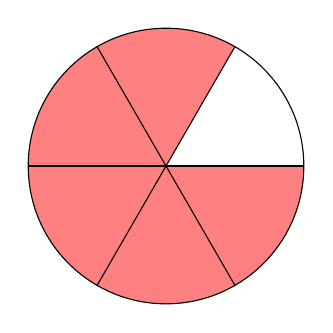
\begin{tikzpicture}[scale=1.75]
		\fill[red!50] (0,0) circle[radius = 1cm];
		\fill[white] (0,0) -- (1cm,0cm) arc (0:60:1cm) -- (0,0);
		\draw (0,0) circle[radius = 1cm];
		\foreach \t in {0,60,120} \draw[rotate=\t] (-1,0) -- (1,0);
	\end{tikzpicture}
	\end{center}
\end{minipage}

\subsection{Multiplying rational numbers}
\index{multiplication!of rational numbers}

Don't worry, your version of the \algebranomicon{} isn't missing any sections. Most textbooks would discuss adding and subtracting rational numbers first, but we're going to start by studying the most helpful of the rational number operations: multiplication.

Suppose that at the cheese market, Knut Krumbli is selling chunks from a 10-pound block of cave-aged goat cheese.\footnote{When cheese is aged in the cool, humid air of underground caves, it can develop a denser texture and a more complex flavor, since small salt crystals form throughout its interior.} Half of the original block of cheese is left, and a local weaver asks to buy three-fourths of it. The original block had a value of 800 Swedish kronor. How much should Knut charge the weaver?

Let's draw a picture. In \cref{fig:fracmult}, the square represents the original block of cheese. We divide the square in half vertically, and the region colored yellow represents how much of the cheese remains. We can then divide the cheese into fourths horizontally and shade in three-fourths (the amount that the weaver wants to buy).

\begin{figure}[!htbp]
\centering
\begin{tikzpicture}
	\draw[fill=yellow!50] (0,0) rectangle (1,2);
	\draw(0,0) rectangle (2,2);

	\draw[fill=yellow!50] (4,0) rectangle (5,2);
	\fill[pattern=north east lines] (4,0) rectangle (5,1.5);
	\draw(5,0)--(5,2);
	\draw[dashed] (4,0.5) -- (5,0.5);
	\draw[dashed] (4,1) -- (5,1);
	\draw[dashed] (4,1.5) -- (5,1.5);
	\draw(4,0) rectangle (6,2);

	\draw[fill=yellow!50] (8,0) rectangle (9,2);
	\fill[pattern=north east lines] (8,0) rectangle (9,1.5);
	\draw(9,0)--(9,2);
	\draw[dashed] (8,0.5) -- (10,0.5);
	\draw[dashed] (8,1) -- (10,1);
	\draw[dashed] (8,1.5) -- (10,1.5);
	\draw(8,0) rectangle (10,2);
\end{tikzpicture}
\caption{Selling three-fourths of one-half of a block of cheese.}
\label{fig:fracmult}
\end{figure}

What fraction of the whole block does this shaded region represent? If we extend the lines, we can see that we've divided up the whole block of cheese into 8 equally-sized pieces. So the weaver is buying $\frac{3}{8}$ of the whole block and Knut should charge 300 kronor.

In the end, we solved a fraction multiplication problem: ``How much is three-fourths of one-half of a whole block of cheese?'' \[\frac{3}{4} \cdot \frac{1}{2} = \frac{3}{8}\] 

\begin{boxdef}[Multiplying rational numbers]
To multiply rational numbers, we multiply numerators to find the numerator of the product. We multiply denominators to find the denominator of the product. \[\frac{a}{b} \cdot \frac{c}{d} = \frac{a \cdot c}{b \cdot d}\]
\end{boxdef}

In the startup exploration for this section, $0 < a < b < 1$, and part (c) asks us to consider $a \cdot b$. Let's think about this from a block-of-cheese perspective. We start with less than a whole block of cheese (since $b$ is less than 1) and we only want to buy a fraction of what's there (since $a$ is less than 1).

So, we are certainly buying less than a whole block of cheese! Since both $a$ and $b$ are less than 1, we know that their product must be less than one.

\subsubsection{Fancy versions of one}

Recall from your elementary school days that any number times 1 is itself. This simple fact, along with the fraction multiplication procedure, gives us an extremely powerful tool that we'll use in various different ways throughout algebra. The key idea is that multiplying something by 1 doesn't change its value, even if we use a ``fancy version of 1''.\footnote{Multiplication by a fancy version of 1 is an application of the identity property of multiplication, which we will study in more detail in \cref{ch:equations}.} Consider, for example:
\begin{commwork}
\frac{5}{8} &=& \dfrac{5}{8} \cdot 1
& multiplication by 1 doesn't change the number
\\[\fracspace]
&=& \frac{5}{8} \cdot \frac{7}{7}
& we can rewrite 1 however we like, here $1 = \frac{7}{7}$
\\[\fracspace]
&=& \frac{35}{56}
& multiply fractions
\end{commwork}

In the end, we have two equivalent fractions $\frac{5}{8} = \frac{35}{56}$. The representation has changed, but the value is the same! The ``fancy one'' we chose here is $\frac{7}{7}$, but any other version of 1 would work the same way: $\frac{-140}{-140}$, $\frac{2\pi}{2\pi}$, $\frac{\sqrt3}{\sqrt3}$\ldots\ The possibilities are endless.

The first application of the ``fancy one'' has to do with one of the themes we encounter throughout algebra: the idea of finding a ``completely simplified'' solution to a problem. Fractions introduce us to the first criteria for something being simplified.

\begin{boxcrit}[Simplified rational numbers \#1]
Fractions should be simplified to \gls{lowest terms}, meaning that the numerator and denominator of the fraction are \gls{relatively prime} integers.
\end{boxcrit}

Two integers are said to be relatively prime (or coprime) if they have no common factors other than 1. So, the fraction $\frac{21}{34}$ is in lowest terms, since the factors of 21 are $\{1, 3, 7, 21\}$ and the factors of 34 are $\{1, 2, 17, 34\}$. They have no factors in common, other than 1.

On the other hand, $\frac{18}{84}$ is not in lowest terms. Both 18 and 84 are even, and so both the numerator and denominator are divisible by at least 2. To write this fraction in lowest terms, we ``undo'' fraction multiplication and search for some fancy ones that we can eliminate: \[\frac{18}{84} = \frac{2 \cdot 3 \cdot 3}{2 \cdot 2 \cdot 3 \cdot 7}  = \frac{2}{2}\cdot\frac{3}{3}\cdot\frac{3}{2\cdot 7} = 1\cdot1\cdot\frac{3}{14} = \frac{3}{14}\]
Once we know how and why this works, we can take a shortcut and ``cancel'' common factors from the numerator and denominator: \[\frac{18}{84} = \frac{2 \cdot 3 \cdot 3}{2 \cdot 2 \cdot 3 \cdot 7}=\frac{\bcancel{2} \cdot \cancel{3} \cdot 3}{\bcancel{2} \cdot 2 \cdot \cancel{3} \cdot 7}  = \frac{3}{2 \cdot 7}\]

\subsubsection{Simplify before you multiply}

We can also use the ``fancy one'' to save ourselves some work! What if we have to multiply:
\[\frac{1}{2} \cdot \frac{2}{3} \cdot \frac{3}{4} \cdot \frac{4}{5} \cdot \frac{5}{6}\]
Let's write the product out ``the long way'' before we actually do any computations. The numerator of the product will be the product of the numerators, and likewise for the denominator:
\[\frac{1}{2} \cdot \frac{2}{3} \cdot \frac{3}{4} \cdot \frac{4}{5} \cdot \frac{5}{6} = \frac{1 \cdot 2 \cdot 3 \cdot 4 \cdot 5}{2 \cdot 3 \cdot 4 \cdot 5 \cdot 6}\]
Then, a common factor in the numerator and denominator is like multiplication by 1, so we can make some simplifications:
\[\frac{1}{2} \cdot \frac{2}{3} \cdot \frac{3}{4} \cdot \frac{4}{5} \cdot \frac{5}{6} = \frac{1 \cdot 2 \cdot 3 \cdot 4 \cdot 5}{2 \cdot 3 \cdot 4 \cdot 5 \cdot 6} = \frac{1 \cdot \cancel{2} \cdot \bcancel{3} \cdot \cancel{4} \cdot \bcancel{5}}{\cancel{2} \cdot \bcancel{3} \cdot \cancel{4} \cdot \bcancel{5} \cdot 6} = \frac{1}{6}\]
The alternative would have been to multiply all of those numbers together by hand and then simplify the fraction to lowest terms\footnote{That would have been $\frac{120}{720}$.}, which is a bunch more work. It pays to be clever!

\begin{boxex}
Multiply: (a)~ $\dfrac{3}{4} \cdot \dfrac{7}{16}$ \qquad (b)~ $\dfrac{15}{8}\cdot\dfrac{4}{7}\cdot\dfrac{14}{3}\cdot\dfrac{1}{5}$

Problem (a) is nothing special. No common factors are shared between numerators and denominators, so we simply multiply as usual.\[\frac{3}{4} \cdot \frac{7}{16} = \frac{3 \cdot 7}{4 \cdot 16} = \frac{21}{64}\] Since there were no common factors to cancel before multiplying, we know the product is already in lowest terms.

To tackle (b), a first helpful step is to factor the individual numerators and denominators to expose all of the factors that are going to be in the product. \[\frac{3\cdot 5}{2 \cdot 2 \cdot 2} \cdot \frac{2 \cdot 2}{7} \cdot \frac{2 \cdot 7}{3} \cdot \frac{1}{5}\]
Then, a common factor in the numerator and denominator is like multiplication by 1, so common factors can be crossed out. Look at what happens in this case!
\[\frac{\cancel{3}\cdot \cancel{5}}{\bcancel{2} \cdot \bcancel{2} \cdot \bcancel{2}} \cdot \frac{\bcancel{2} \cdot \bcancel{2}}{\bcancel{7}} \cdot \frac{\bcancel{2} \cdot \bcancel{7}}{\cancel{3}} \cdot \frac{1}{\cancel{5}} = 1\]
Note that all of the factors cancel out in the denominator. A common mistake at this point is to replace the ``empty'' denominator with 0 -- but remember, a common factor in the numerator and denominator is like a factor of 1, which is the fraction $\frac{1}{1}$, not $\frac{1}{0}$, so there's always a ``phantom one'' lurking there even if we don't write it.
\end{boxex}

\subsection{Adding and subtracting rational numbers}
\index{addition!of rational numbers}
\index{subtraction!of rational numbers}

Knut Krumbli would tell you that bringing together a herd of 8 goats and a herd of 11 goats results in a herd of 19 goats. It's goat herding, not rocket science.

But, combining a herd of 4 goats and a flock of 13 sheep doesn't really give us 17 of anything until we can find some shared characteristic that is common to both groups. For instance, we could say we have a group of ``17 mammals'' or ``17 quadrupeds''.

So it goes with fractions. When our fractions have a shared name (a common denominator) we can total up how many things we have with that name: 8 thirds and 11 thirds makes 19 thirds. In math symbols, we write
\[\frac{8}{3} + \frac{11}{3} = \frac{19}{3}\]
On the other hand, when our quantities \textit{don't} share a common unit (a common denominator), we have to find one before we can add in a meaningful way.

Given a fraction, we can use multiplication by a ``fancy one'' to generate a new fraction that has the same value but a different, perhaps more helpful, denominator.

Some people like to try and find the \textit{least common denominator}, but that's not strictly necessary. Any common denominator will do. In fact, a guaranteed common denominator of any two fractions is the \textit{product of their denominators}.

\begin{boxdef}[Adding and subtracting rational numbers]
To add rational numbers, we must have a common denominator, for example the product of the original denominators. Then we add the numerators, and keep the common denominator.
\[\frac{a}{b} + \frac{c}{d}
= \frac{a\cdot d + b\cdot c}{b\cdot d}\]
To subtract rational numbers, change the subtraction problem to an ``addition of the opposite'' problem and then follow the algorithm for addition.

Here's the derivation of fraction addition in a bit more detail. Note how we use multiplication by 1 to find a common denominator $b \cdot d$:
\[\frac{a}{b} + \frac{c}{d}
= \left( \frac{a}{b}\cdot 1 \right) + \left( 1\cdot\frac{c}{d} \right)
= \left( \frac{a}{b}\cdot\frac{d}{d} \right) + \left( \frac{b}{b}\cdot\frac{c}{d} \right)
= \frac{a\cdot d}{b\cdot d} + \frac{b\cdot c}{b\cdot d}
= \frac{a\cdot d + b\cdot c}{b\cdot d}\]

\end{boxdef}

\subsubsection{Negative fractions}

Where should we put the negative sign when we have a negative fraction? Does it matter? Consider the following three possibilities. Are they all equivalent?
\[ -\frac{3}{4} \qquad \frac{-3}{4} \qquad \frac{3}{-4}\]
A fraction is a way of writing a division problem. If Knut's four children share three bowls of lingonberries equally, then each child will get $3\div4 = \frac{3}{4}$ of a bowl of berries.\footnote{Lingonberries are a popular fruit in Scandinavia and throughout northern, central, and eastern Europe. The berries are quite tart, and so they are usually mixed with sugar and preserved as jam or compote. In Sweden and Norway, reindeer is traditionally served with gravy and lingonberry sauce. Yes, Scandinavians eat reindeer.} The fraction $\frac{3}{4}$ is just another way of writing $3 \div 4$. So, all three of the fractions above have the same value.

In the first example, the whole fraction has been negated. In the second and third examples, the numbers have opposite signs and so the quotient will be negative. In other words it actually doesn't matter where we put the negative sign. We can put it where it is most convenient for the problem. Very often, that's in the numerator of the fraction.

\subsubsection{Mixed numbers}

Improper fractions have a numerator that is greater than or equal (in absolute value) to their denominator, like $\frac{5}{3}$ or $\frac{-84}{16}$. Improper fractions have been scorned by many elementary school mathematics teachers, who instead prefer mixed numbers: $1\frac{2}{3}$ or $-5\frac{1}{4}$. But, improper fractions are often much easier to work with than mixed numbers.\footnote{One situation where improper fractions are superior is when describing the slope of a line, as we will see in \cref{ch:linear}.}

\begin{boxcrit}[Simplified rational numbers \#2]
Simplified \glspl{improper fraction} are preferred over \glspl{mixed number} and decimals. Only convert to a mixed number or decimal when the context (or the directions) require it.
\end{boxcrit}

We usually prefer exact fraction answers over decimal approximations. Writing the decimal $\frac{10}{7}$, for instance, is much preferred over $1.43$, and it's better even than the exact answer $1.\overline{428571}$ (yep, that's a big chuck o' repeating decimal).

But, be sure to read questions carefully! There are exceptions to these rules. When working in a real-world context, a certain number format may make more sense. For example, when solving a problem about money, the answer \$3.50 makes a lot more sense than $\$\frac{7}{2}$. Likewise, the answer ``$1\frac{1}{3}$~pounds of cheese'' is better than ``$\frac{4}{3}$~pounds of cheese''. In ambiguous cases, we will make it clear what number format is preferred.

When faced with mixed numbers in a problem, we have to be careful. When adding, we can convert all mixed numbers to improper fractions, or work with them ``as is''. Subtracting with mixed numbers is tricky, however, because we we may have to handle regrouping. Multiplication is even trickier.

Since we prefer improper fractions as final answers anyway, we recommend converting all mixed numbers to improper fractions before starting computations. To convert a mixed number to an improper fraction, all we have to do is think about the mixed number as an addition problem:
\[3\frac{5}{8} = 3 + \frac{5}{8} = \frac{3}{1} + \frac{5}{8} = \frac{3 \cdot 8 + 1 \cdot 5}{1 \cdot 8} = \frac{24 + 5}{8} = \frac{29}{8}\]
Here we used the fact that any integer has a ``phantom one'' in its denominator: $3 = \frac{3}{1}$. We don't usually write it, but it's there when we need it.

\begin{boxex}
Compute each of the following:

\begin{enumerate}[itemsep=10pt]
\item \onerowex{$\dfrac{3}{4} + \dfrac{5}{6}$}{These fractions do not have a common denominator, so we'll have to find one. We could use their least common denominator (which is 12) or use the product of the denominators (which is 24). Let's use 24: \[\dfrac{3}{4} + \dfrac{5}{6} = \dfrac{3 \cdot 6 + 4 \cdot 5}{4 \cdot 6} = \dfrac{18 + 20}{24} = \dfrac{38}{24} = \dfrac{19}{12}\]}

\item \onerowex{$1\dfrac{2}{5} - 1\dfrac{7}{8}$}{First, we'll convert to improper fractions and change the subtraction to addition-of-the-opposite, putting the negative sign in the numerator of the fraction. Then we add. In the end, we can adjust the negative sign again: \[\dfrac{7}{5} - \dfrac{15}{8} = \dfrac{7}{5} + \dfrac{\umin15}{8} = \dfrac{7 \cdot 8 + 5 \cdot \umin15}{5 \cdot 8} = \dfrac{56 + \umin75}{40} = \dfrac{\umin19}{40} = -\dfrac{19}{40}\]}
\end{enumerate}
\end{boxex}

In the startup exploration for this section, $0 < a < b < 1$. Part (a) asks about $a + b$. Since both numbers are positive, their sum is positive, but we don't have enough information to tell whether the sum is greater than 1. If $a$ and $b$ are both less than $\frac{1}{2}$, for example, then their sum will be less than 1. On the other hand, if they are both greater than $\frac{1}{2}$, then their sum will be greater than 1.

Part (b) asks us to consider $a - b$. Since $a$ is less than $b$, we're subtracting a larger number from a smaller number, and so the answer must be negative.

We can reason this out in another way: $a-b$ is the same as $a + (\umin b)$. The absolute value of $b$ is the same as the absolute value of $\umin b$. And so this sum will be negative because the negative number is the one with the greater absolute value. In any case, $a-b$ is negative and so we know for sure that it is less than 1.

\subsection{Dividing rational numbers}
\index{division!of rational numbers}

Fraction division may be the most poorly understood operation in all of arithmetic. The algorithm for dividing fractions seems arbitrary, and it's often difficult to judge whether our answers make sense. Let's pause for a moment to think about what fraction division means.

Suppose Jorunn Krumbli, Knut's wife, is making scarves for the goats (Scandinavian winters are chilly). She has 8 meters of burlap, and each scarf requires $\frac{3}{4}$ of a meter. How many scarves can she make?

\kverse{Meet Jorunn Krumbli, Knut's wife, great-great-great-grandmother.}

This question is asking us to compute $8 \div \frac{3}{4}$, but let's try to solve the problem by drawing a picture. Suppose this rectangle represents Jorunn's 8 meters of burlap.
\begin{center}

\begin{tikzpicture}
	\foreach \x in {0,2,...,14} \draw (\x,0) rectangle (\x+2,1);
\end{tikzpicture}
\end{center}

To figure out how many pieces of $\frac{3}{4}$ meter are in there, let's first determine the number of pieces of size $\frac{1}{4}$ meter. To do that, we'll break each meter into four pieces. That gives us $8 \cdot 4 = 32$ pieces total.
\begin{center}
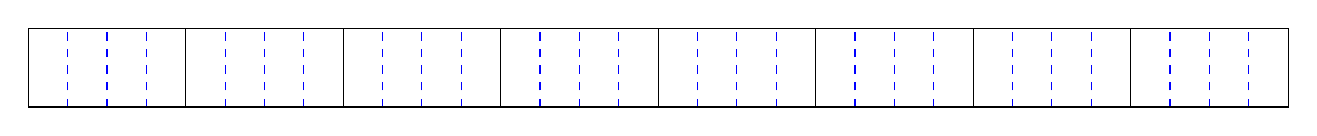
\begin{tikzpicture}
	\foreach \x in {0,0.5,...,15.5} \draw[blue,dashed] (\x,0) -- (\x,1);
	\foreach \x in {0,2,...,14} \draw (\x,0) rectangle (\x+2,1);
\end{tikzpicture}
\end{center}

Now, let's gather these pieces up into groups of three. We'll be able to make 10 whole groups, and we'll have 2 pieces left over. Since we have two pieces, but need three, we have $\frac{2}{3}$ of a group. So, Jorunn can make $10\frac{2}{3}$ scarves for the goats.
\begin{center}
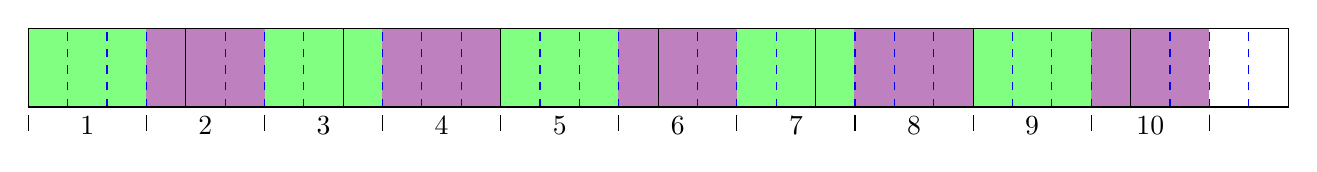
\begin{tikzpicture}
	\foreach \x in {1.5,4.5,...,13.5} \draw[white,fill=violet!50] (\x,0) rectangle (\x+1.5,1);
	\foreach \x in {0,3,...,12} \draw[violet!50, fill=green!50] (\x,0) rectangle (\x+1.5,1);
	\foreach \x in {1,...,10} {
		\draw (1.5*\x-1.5, -.1) -- (1.5*\x-1.5, -.3);
		\draw (15, -.1) -- (15, -.3);
		\draw (1.5*\x-0.75,0) node[below]{\x};
	}
	\foreach \x in {0,0.5,...,15.5} \draw[blue,dashed] (\x,0) -- (\x,1);
	\foreach \x in {0,2,...,14} \draw (\x,0) rectangle (\x+2,1);
\end{tikzpicture}
\end{center}

Let's retrace our steps. We set out to solve $8 \div \frac{3}{4}$, but in our picture we first multiplied to find the total number of fourths, and then we divided to find how many groups of three we could make. In other words: $8 \div \frac{3}{4}$ must have the same answer as $8 \cdot \frac{4}{3}$. Does that look familiar?

\begin{boxdef}[Dividing rational numbers]
Dividing by a number is the same as multiplying by the reciprocal of the number. So, we can change a given fraction division problem into an equivalent fraction multiplication problem and then use the rules for fraction multiplication. \[\frac{a}{b} \div \frac{c}{d} = \frac{a}{b} \cdot \frac{d}{c} = \frac{a \cdot d}{b \cdot c}\]
\end{boxdef}

Recall that the \gls{reciprocal} of a fraction is the fraction that interchanges the numerator and the denominator of the original fraction. The reciprocal of an integer (which is sitting on a phantom 1) is ``one over the original integer''.

\begin{boxex}
Compute each of the following:

\begin{enumerate}[itemsep=10pt]
\item \onerowex{$\dfrac{5}{6} \div -\dfrac{3}{4}$}{We don't need a common denominator or anything, so we can just jump right in with fraction division. We don't even need to move the negative sign, since we know the answer will be negative. \[\dfrac{5}{6} \div -\dfrac{3}{4} = \dfrac{5}{6} \cdot -\dfrac{4}{3} = -\dfrac{20}{18} = -\dfrac{10}{9}\]}

\item \onerowex{$3\dfrac{3}{4} \div 5$}{First, we'll convert to improper fractions, then we'll carry out fraction division At the end, we can simplify before we multiply! \[3\dfrac{3}{4} \div 5 = \dfrac{15}{4} \div \dfrac{5}{1} = \dfrac{15}{4} \cdot \dfrac{1}{5} = \dfrac{3 \cdot 5}{4} \cdot \dfrac{1}{5} = \dfrac{3 \cdot \cancel{5}}{4} \cdot \dfrac{1}{\cancel{5}} = \dfrac{3}{4}\]}
\end{enumerate}
Let's think about this last answer for a second: does it makes sense? Look again at the problem we were given. If we interpret this as the question``how many groups of 5 are in $3\frac{3}{4}$?'', then we can see that we can't even make one whole group: $3\frac{3}{4}$ is less than 5! So, it makes sense for our answer to be less than 1.
\end{boxex}

\subsubsection{Fractions inside fractions}

As if fractions on their own weren't enough, you may soon face the \gls{turducken}\footnote{A ``turducken'' is a food product where a deboned chicken is stuffed inside a deboned duck, which is then stuffed inside a deboned turkey. In culinary terminology, this is an example of ``engastration'', a cooking method in which one animal is stuffed inside the gastric cavity of another\ldots\ which is probably yet another phenomenon that you didn't know had a name.} of arithmetic, the dreaded ``fraction in a fraction''. Note that a fraction-in-a-fraction would not be considered simplified since the criteria state that the numerator and denominator must be \textit{integers}.

These creatures can look hard to handle, but don't be intimidated. Recall that a fraction is just a division problem. So, we can rewrite things using a division sign and divide as usual.\footnote{The fancy mathematical name for the $\div$ symbol is \gls{obelus} (plural: obeli)\ldots\ another thing that you probably didn't know had a name.}

\begin{boxex}
Simplify each of the following:

\begin{enumerate}[itemsep=10pt]
\item \onerowex{$\dfrac{~~4~~}{\left( \frac{1}{3} \right)}$}{All we have to do is rewrite the fraction-in-a-fraction as ``numerator $\div$ denominator'', and then divide as usual. \[\dfrac{~~4~~}{\left( \frac{1}{3} \right)} = 4 \div \dfrac{1}{3} = \frac{4}{1} \div \frac{1}{3}= \frac{4}{1} \cdot \dfrac{3}{1} = 4 \cdot 3 = 12\]}

\item \onerowex{$\dfrac{~~\left( \frac{2}{5} \right)~~}{\left( 1\frac{3}{8} \right)}$}{Here we rewrite using the obelus, then convert to improper fractions, then divide! \[\dfrac{~~\left( \frac{2}{5} \right)~~}{\left( 1\frac{3}{8} \right)} = \dfrac{2}{5} \div 1\dfrac{3}{8} = \dfrac{2}{5} \div \dfrac{11}{8} =\dfrac{2}{5} \cdot \dfrac{8}{11} = \dfrac{16}{55}\]}
\end{enumerate}
\end{boxex}

In the startup exploration for this section, we have rational numbers $a$ and $b$ where $0 < a < b < 1$. Part (d) asks us to consider $a \div b$. This division problem is another way of writing $\frac{a}{b}$. Since $a$ is less than $b$, we know that this fraction is a proper fraction (as opposed to an improper fraction), which means it is less than 1. So, $a \div b$ is less than 1.

\subsection{Evil and Wrong}

Everyone makes mistakes, but not all mistakes are created equal. Some mistakes are not just wrong, the are \evilandwrong. ``Wrong'' because they are mistakes, ``evil'' because they are subtle, and sneaky, and tempting.

What we mean here is that sometimes we feel drawn to perform certain arithmetic or algebraic maneuvers which seem so logical, so easy, so natural, so tempting\ldots\ but which in reality are a total trap. For example:

\begin{boxwarn}
Armed with the idea of ``simplify before you multiply'', we might want to try and pull this stunt in other places: \[\frac{2+3}{2+7} = \frac{\bcancel{2}+3}{\bcancel{2}+7} = \frac{3}{7}\]Seems logical, right? But so wrong! There is no ``simplify before you add'' maneuver, tempting though it may be. Such a thing is \evilandwrong.
\end{boxwarn}

You may be thinking, ``Nah, I'd never to that,'' and with numerical expressions like these, you may be right. But later, when faced with variable expressions like \[\frac{x+3}{x+7},\]
this temptation may come back, in disguise. We'll draw attention to these \evilandwrong{} mistakes as we go along because they are so tempting. Beware!


% % % % % % % % % % % % % % % % % % % % % % % % % % % % % % % % % % % % % % % % 
\section{Order of operations}
\label{sec:orderofops}

We turn now to something else that it probably familiar, the \gls{order of operations}. Consider the following problem as we get started:

\begin{boxexplore}[Who's right?]
The four Krumbli kids each performed the following computation: \[14 - 6 \cdot 7 + 10\] Sini got $\umin38$,
Siri got $\umin18$,
Sten got $66$,
and Stig got $136$. Which of them performed the computation correctly? What mistakes did the others make?
\end{boxexplore}

\kverse{Meet the Krumbli children: Sini, Siri, Sten, and Stig.}

The order of operations gives us a standard procedure for simplifying numeric expressions. A \gls{numeric expression} is the algebra way of describing something you may have called just a ``math problem'' in elementary school. For example, $12 - 5$ is a numeric expression. It is not in its simplest form because we can evaluate $12 - 5$ and write 7 instead.  

\begin{boxcrit}[Simplification rule \#1]
A numeric expression is completely simplified if all operations have been evaluated and all grouping symbols have been eliminated. The resulting quantity is called the \textit{value} of the expression.
\end{boxcrit}

As we go along in algebra, we will learn many rules that maintain ``mathematical equivalence''.  Expressions are mathematically equivalent if they represent the same quantity.  For example, $\frac{4}{8}$ is equivalent to $\frac{1}{2}$, and $12 - 5$ is equivalent to 7. Our job when we simplify an expression is to ensure that we maintain equivalence from one step to the next. The order of operations is a set of rules for how to do that.

\begin{boxdef}[Order of operations]
An agreed-upon order for simplifying numeric expressions. The big idea is that ``more powerful'' operations take priority over ``less powerful'' operations. When we want to alter the usual rules of precedence, we introduce grouping symbols to make our intentions clear.

When simplifying an expression, we evaluate things in the following order:\footnote{PEMDAS is an mnemonic acronym for remembering the order of operations: Parentheses, Exponents, Multiplication, Division, Addition, Subtraction. In Canada it's BEDMAS (B for Brackets). In the UK and Australia it's BIDMAS or BODMAS (for Indices and Orders, which are other words for exponent). A better acronym might be GEMS or PEMA, which group together the pairs of operations that have the same priority (the G is for Grouping symbols).}

\begin{description}
\item[First:] Grouping symbols like (parentheses) and [square brackets], as well as other subtle grouping symbols like absolute value and the vinculum. Here we work from the innermost set of groupers\footnote{As in ``grouping symbols'', not the fish.} to the outermost.

\item[Then:] Exponents (later, we will include roots and logarithms at this level of the hierarchy). In the case of a ``stack'' of exponents, work from the top down.

\item[Then:] Multiplication and division. Recall that dividing is the same as ``multiplying by the reciprocal''. So, these two operations have the same priority and we work from left to right.

\item[Finally:] Addition and subtraction. Recall that ``subtracting'' is the same as ``adding the opposite''. So, these two operations have the same priority, and we work from left to right.
\end{description}
\end{boxdef}

\begin{boxex}
\label{ex:workdown}
Simplify: $14 - 6 \cdot 7 + 10$

\exsoln\ The correct answer follows the order of operations, like so:
\begin{commwork}
14 - 6 \cdot 7 + 10 &=& 14 - 42 + 10
& work mult'n before addition or subtraction
\\
&=&\umin28 + 10
& work add'n and sub'n left to right
\\
&=&\umin18
\end{commwork}%
This is the problem from the startup exploration, so it is Siri who had the right answer.

Students who just memorize a clever mnemonic device might be tempted to do the \underline{A}ddition before the \underline{S}ubtraction, but don't be fooled! Those two operations have the same priority. (Sini made this mistake and got $\umin38$.)

Sten worked the operations straight through from left to right, all at the same priority and got 66. Stig did something very, ahem, ``creative'': $(14-6)\cdot(7+10) = 8 \cdot 17 = 136$.
\end{boxex}

Notice how we showed the work going down the page, simplifying the problem one step at a time. Some people prefer to work across the page, and that's okay too. The point is that it's important to show work in an organized way when we solve a problem so that our reasoning and thought process are clear.

%\[\begin{aligned}
%	&~ 14 - 6 \cdot 7 + 10\\
%=	&~ 14 - 42 + 10
%&& \quad\text{work multiplication before addition/subtraction}\\
%=	&~ \umin28 + 10
%&& \quad\text{work addition and subtraction from left to right}\\
%=	&~ \umin18
%\end{aligned}\]

%\addtodoitem{Criteria for showing work.}

The work we show is the road map to our solution. Whoever reads over our work must be able to follow and understand our steps, without having to make any assumptions about what we actually did to reach our answer. It's a bad habit to skip steps, and it's no help to people reading our work to claim that we did a step in our head. Every step we take needs to be written down clearly and neatly.

\begin{boxwarn}[Abuse of the equal sign]
Consider the following work, written out by a student to simplify $8 \cdot 4 + 10$ \[8 \cdot 4 = 32 + 10 = 42 \qquad\text{OK or not OK?}\]
The student has reached the correct value, and it may even be clear what the student is thinking: ``8 times 4 is 32, plus 10 more makes 42''. This, however, is a heinous abuse of the equal sign! Look at what the first part of the work says: \[8 \cdot 4 = 32 + 10 \qquad\text{These are not equal!}\]
One way to avoid this misuse of the equal sign is to write your work going down the page (as shown in \cref{ex:workdown}). If you prefer to write across the page, be sure to write out the whole problem as you perform each simplification: \[8 \cdot 4 + 10 = 32 + 10 = 42\]
\end{boxwarn}

In the next few sections, we'll look more closely at some trickier aspects of the order of operations.

\subsection{About grouping symbols}

As expressions get complicated, we may have grouping symbols inside of other grouping symbols. If we have different symbols (like parentheses with [some bracketed expression] inside), we can more easily see where different groups begin and end. But, we may just find a bunch of parentheses, like in the example below. In that case, we have to be a bit careful about what's being grouped together.

\begin{boxex}
Simplify: $12+(3-(4-2)+5)$

\exsoln\ When faced with multiple grouping symbols, we must start with the innermost set of grouping symbols and evaluate our way to the outermost. Once we have simplified the expression inside a set of grouping symbols down to a single quantity, we can write that quantity without the groupers.
\begin{commwork}
12+(3-(4-2)+5) &=& 12+(3-2+5)
\\
&=& 12+(1+5)
\\
&=& 12+6
\\
&=& 18
\end{commwork}

%\[\begin{aligned}
%	&~ 12+(3-(4-2)+5)\\
%=	&~ 12+(3-2+5)\\
%=	&~ 12+(1+5)\\
%=	&~ 12+6\\
%=	&~ 18
%\end{aligned}\]
\end{boxex}

\subsubsection{The vinculum is a grouping symbol}

The \gls{vinculum}, as in the fraction bar, is a grouping symbol. For example, if the task is to simplify a fraction such as:
\[\frac{20+2^2\cdot(14-9)}{(2-4)^3},\]
then we must think of the expression in the numerator as a group, and likewise for the denominator. In other words, like so: \[\Bigl(20+2^2\cdot(14-9)\Bigr)\div\Bigl((2-4)^3\Bigr).\]

We have two options for simplifying this. We might keep it in a fraction the whole time, or we could simplify the numerator and denominator separately and then squish them back into a fraction at the end.

\begin{boxex}
Simplify: $\dfrac{20+2^2\cdot(14-9)}{(2-4)^3}$

\exsoln\ Let's dismantle this thing and handle it in two pieces. The numerator works like this:
\begin{commwork}
20 + 2^2 \cdot (14-9) &=& 20 + 2^2 \cdot 5\\
&=& 20 + 4 \cdot 5\\
&=& 20 + 20\\
&=& 40
\end{commwork}%
The denominator works like this: $(2-4)^3 = (\umin2)^3 = \umin8$. Then, we can put the pieces back into their original fraction configuration:\[\dfrac{20+2^2\cdot(14-9)}{(2-4)^3} = \dfrac{40}{\umin8} = \umin5\]
\end{boxex}

\subsection{About exponents}

An expression of the form $a^b$ is read ``$a$ to the power of $b$'' or ``$a$ to the $b^{\text{th}}$ power''. In such an expression, $a$ is called the \gls{base} and $b$ is called the \gls{exponent}. We call the whole thing a \gls{power} of $a$, since $a$ is the base.

We will get into more detail about exponents later on, but we'll pause here to mention two key ideas. First, recall that we can think about an exponent as shorthand for a repeated multiplication.\footnote{As with ``multiplication is repeated addition'', this interpretation breaks down eventually. Expressions like $5^{-3}$ and $16^{1/2}$ don't really translate well into ``repeated multiplication''. Don't panic about the idea of a negative number or a fraction up there in the exponent! All will be revealed in time.}
\[a^b = \underbrace{a \cdot a \cdot a \dotsb a}_{\text{$b$ times}}\]
That part you probably knew already. This next fact may be new:

\begin{boxdef}[Raising to the power zero]
For any nonzero number $a$, the expression $a^0 = 1$. In other words, any nonzero number raised to the power 0 equals 1.
\end{boxdef}

When we say here that $a$ is a ``nonzero number'' this means, naturally enough, that $a$ cannot be 0. The expression $0^0 \neq 1$. What \textit{does} it equal? That's a tricky question that will have to wait for later. $0^0 $ is an unusual mathematical creature!\footnote{It's not the only one, either. In 1872, Karl Weierstrass (or Weierstra\ss, if you prefer the German double-S) shook the foundations of calculus with his mathematical monster, now called the ``Weierstra\ss{} function''. It's a bit complicated to get into the details, but it made some other mathematicians very upset. Drama!}

We'll get into the ``hows and whys'' of exponents in \cref{ch:expofunc,,ch:expoexpr}, and we'll return to the idea of the zero exponent. In the meantime, here's an example of how this fact might come in handy.

\begin{boxex}
Simplify: $\left( \dfrac{120-(24-5^2)}{7^2 \cdot 400 \div 6^3} \right)^0$

\exsoln If we go on ``auto-pilot'' we might follow all of the simplification rules, work from the inside to the outside, simplify the numerator, simplify the denominator\ldots

But, the expression is raised to the power 0. So the answer is probably 1! We must check that we don't have $0^0$, but we can use a little number sense to do a quick check of the numerator in the fraction, and see that it will not equal zero. (Can you see why without having to work it all out?)

We must also check that the denominator is not zero. A quick check there shows that it is not zero either. (Can you see why?) So, this one's easy:
\[\left( \frac{120-(24-5^2)}{7^2 \cdot 400 \div 6^3} \right)^0 = 1\]
\end{boxex}

The lesson here is to look at the entire problem and plan an efficient solution strategy \textit{before} just jumping in and crunching numbers. In this case, we can save ourselves a lot of work with a bit of careful observation.

\subsubsection{Fractions versus exponents}

If we have a fraction raised to a power, we must be very mindful of the notation and to what, exactly, the exponent applies.

\begin{boxex}
Simplify each of the following:

\begin{enumerate}[itemsep=10pt]
\item \onerowex{$\left( \dfrac{~2~}{~3~} \right)^4$}{The parentheses indicate that we are multiplying together 4 copies of the fraction:\[\left( \dfrac{~2~}{~3~} \right)^4 = \left( \dfrac{~2~}{~3~} \right)\left( \dfrac{~2~}{~3~} \right)\left( \dfrac{~2~}{~3~} \right)\left( \dfrac{~2~}{~3~} \right) = \dfrac{~16~}{~81~}\]}

\item \onerowex{$\dfrac{~2\,^4}{~3~~}$}{Remember that the numerator is a group, and so the exponent applies only to the 2, not the whole fraction:\[\dfrac{~2\,^4}{~3~~} = \dfrac{~2\cdot2\cdot2\cdot2~}{~3~} = \dfrac{~16~}{~3~}\]}
\end{enumerate}
\end{boxex}

Keep this last example in mind when writing your own expressions, as well. Our notation must match our intentions. What exactly do we intend the exponent to apply to? Do we need to add parentheses to make our intentions clear?

\subsubsection{One of the trickiest concepts in Algebra 1}

What is the difference between the following three expressions? \[(\umin3)^2 \qquad \umin(3^2) \qquad \umin3^2\]
Tricky, right? This is an important difference that will come back over and over again, and it will look a little different every time.

In the first case, the parentheses make it clear: $(\umin3)^2$ means ``raise negative three to the second power''.
\[(\umin3)^2 = \umin3 \cdot \umin3 = 9\]
As usual, the product of two negatives is positive (Hitler gets hit by a truck). The second case is clear as well. The parentheses indicate that we should simplify the exponent first and then take the opposite of the result:
\[\umin(3^2) = \umin(3\cdot3) = \umin(9) = \umin9\]

The third case, $\umin3^2$,  is the tricky one. It looks kind of ambiguous, since there are no parentheses. But, we can interpret $\umin3$ as the product $\umin1\cdot3$. In this case, we have
\[-3^2 = \umin1\cdot3^2 = \umin1\cdot9 = \umin9\]
Now, it's clear what to do even without the parentheses, and that is the key.

\begin{boxdef}[Opposites of numbers to a power]
The expression $-a^n$, written without parentheses, is equivalent to the parenthesized expression $-(a^n)$. For example: $-3^2 = -(3^2) = -9$.
\end{boxdef}

You might be saying to yourself, ``No sweat. I get it.'' But (if history and human nature are any indication) you may find yourself tripping over this concept at some point. Confusion around the notation can pop up, for instance, when we're typing expressions into a graphing calculator.\footnote{A note to old-school parents who are used to working with calculators that use reverse Polish notation (RPN) or a stack, and might want to argue that $-3^2 = 9$. When using an RPN calculator we punch in $-3$ and press enter to push that quantity onto the stack. The number and the negative are both in the stack together, so squaring the entry on the top of the stack means squaring negative three, which is equivalent to $(-3)^2$ and not the same as $-3^2$.}

\subsection{About multiplication}

In algebra we frequently use $x$ (the letter) to stand for a unknown or variable quantity. So, we never use $\times$ to show multiplication. It would be too confusing to have a mix of letter-$x$'s and multiplication-$\times$'s in the same expression. Can you imagine trying to decode something like: \[x \times 3 + 4 \times x = x + 4 x \times x \times x \text{\qquad Yikes!}\]

\begin{boxwarn}[No more x for multiplication!]
To show the operation of multiplication, use an asterisk, a dot, or parentheses. Instead of writing $3\times 4$ to represent ``3 times 4'', we write: $\,3 \ast 4$, or $\,3 \cdot 4$, or $\,3(4)$.
\end{boxwarn}

\subsubsection{Implied operations}

A key aspect of algebra will be learning to read the notation and use it correctly when writing expressions and equations. Algebra is very much like a language, and all languages have special rules. For example, in English we sometimes smash up two words as a contraction: instead of writing ``do not'' we can write ``don't''.

We used contractions (of a kind) in mathematics as well. We don't usually write a positive sign in front of positive numbers. We don't usually write the phantom 1 that is in the denominator of an integer.

Another kind of mathematical contraction is the use of an \gls{implied operation}. This arises most often when dealing with multiplication. Here's an example of how implied operations can sneak into a problem.

\begin{boxex}
Simplify: $12 - 5(2 + 8)$

\exsoln\ Be on the lookout for implied operations!
\begin{commwork}
12-5(2+8) &=& 12-5(10)
& add in the parentheses first
\\
&=& 12-50
& that 5(10) means mult'n, and must happen first!
\\
&=& \umin38\\
\end{commwork}%
A very common mistake in the second step is to do the $12-5$ first, instead of the $5(10)$. But that would violate the order of operations!
\end{boxex}

% % % % % % % % % % % % % % % % % % % % % % % % % % % % % % % % % % % % % % % % 
\chaptersummary

In this chapter we have thought deeply about fundamental ideas regarding numbers and operations. This exploration has perhaps presented some familiar ideas in a new light. Prepare to see more of this! One of the fun and surprising things about mathematics is that we can often learn something new from looking at a familiar concept in a different way. 

Here, we looked closely at two important sets of numbers -- the integers and the rational numbers -- and at our first example of simplification using the order of operations. Armed with this knowledge, we now venture deeper into the algebraic wilderness. Onward!
